
\chapter{Pruebas de funcionamiento}

Para revisar el buen funcionamiento de la aplicación desarrollada, se utilizó el software dispuesto por Apple Inc,  el entorno de desarrollo Xcode y herramientas asociadas. Para obtener estas aplicaciones, es necesario poseer una cuenta de desarrollador para \textbf{iOS} o \textbf{Mac OS X}, las cuales se pueden obtener en el sitio web \url{https://developer.apple.com/programs/} luego de pagar la matrícula impuesta.\\

La cuenta de desarrollador permite acceso al repositorio de herramientas \cite{apple-repositorio} y también acceso a versiones de los sistemas operativos antes de lanzamiento.
Además permite poner a la venta las aplicaciones desarrolladas en la \textit{\textbf{App Store}}\cite{apple-appstore}.

% datos en el camino, seguimiento de un tweet, pantallazos de debug
\section{Cambio de tiempo y/o canal}

Las primeras pruebas estuvieron relacionadas con el cambio de tiempo a través de peticiones al dispatcher con argumentos en la cadena de consulta, estas se realizaron con la aplicación de OS X: \textbf{Quicktime X}, la cual permite reproducir streams que cumplen con las especificaciones de HTTP Live Streaming. Otra alternativa que además se encuentra disponible en otros sistemas operativos es \textbf{VideoLan VLC}. Las pruebas consistieron en modificar los argumentos \textbf{t}, \textbf{s} y \textbf{c} de URLs del tipo:
\url{http://ssdemo.altavoz.net/playlist/playlist.m3u8?s=tvn&t=1353186024&c=0}, donde el parámetro \textbf{t} corresponde al tiempo Unix del 17 de noviembre de 2012 18:00:24 GMT-3.\\

El especificar el tiempo en el parámetro \textbf{t} resulta siempre en una lista de reproducción con segmentos asociados al tiempo correspondiente. Además se monitoreó la respuesta a través de la aplicación rastreadora de paquetes Wireshark. Para esto se necesitó aplicar un filtro especial de forma que los paquetes relacionados con HTTP Live Streaming fueran entregados. El filtro corresponde a mostrar paquetes recibidos desde el servidor donde el cliente, en este caso Quicktime, se contacta para obtener una lista de reproducción, y además pedir la entrega de paquetes que tengan en su contenido la palabra \textbf{apple}.

\begin{figure}[H]
	\centering
\begin{lstlisting}
		ip.addr==200.91.44.49 && http contains apple
\end{lstlisting}
\caption{Filtro en Wireshark que muestra sólo paquetes relacionados con el HLS}
\end{figure}


Los resultados obtenidos son los esperados y corresponden a la reproducción del video en el momento indicado y en el canal indicado según los parámetros.

\begin{figure}[H]
	\centering
	\begin{tabular}{cc}
	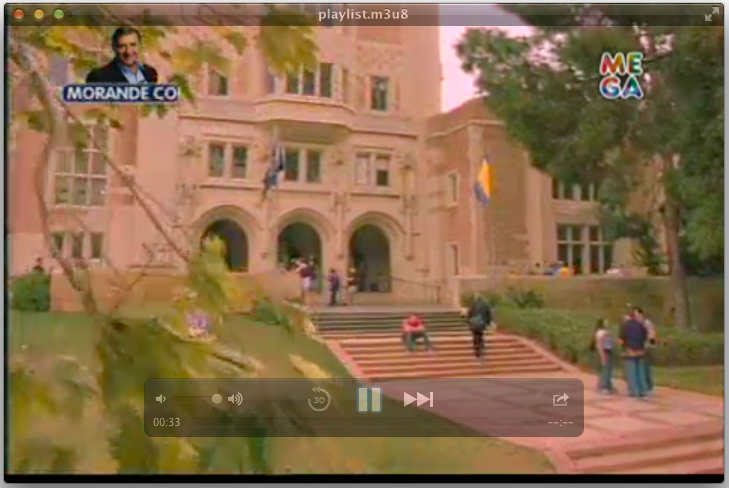
\includegraphics[scale=0.3]{imgs/qt-mega.png} & 
	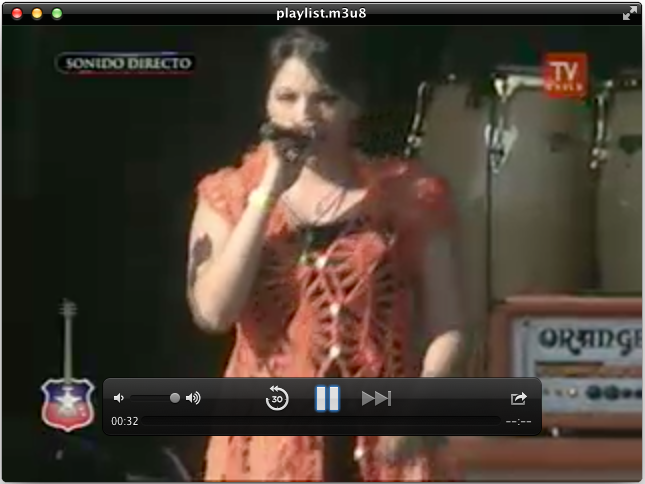
\includegraphics[scale=0.3]{imgs/qt-tvn.png} \\
	\end{tabular}
	\caption{Captura de Quicktime reproduciendo lista de reproducción a través de un URL.}
	\label{qt-tvn-mega}
\end{figure}

Utilizando \textbf{Wireshark} se observaron los datos entregados al cliente desde el servidor como \textit{\textbf{cookies}} indicadas en \ref{subsec:cookies}.

\begin{figure}[H]
	\centering
\begin{lstlisting}
HTTP/1.1 200 OK
Server: nginx/1.2.0
Date: Sat, 24 Nov 2012 18:06:10 GMT
Content-Type: application/vnd.apple.mpegurl
Transfer-Encoding: chunked
Connection: keep-alive
Keep-Alive: timeout=20
X-Powered-By: PHP/5.3.15-1~dotdeb.0
Set-Cookie: stream=tvn
Set-Cookie: t0=1353186024
Set-Cookie: tp=1353780370
Set-Cookie: ti=1353186033
Set-Cookie: tl=1353186085
Set-Cookie: si=1
Set-Cookie: sf=6

#EXTM3U
#EXT-X-TARGETDURATION:10
#EXT-X-PROGRAM-DATE-TIME:2012-11-17T18:00:33-03:00
#EXT-X-VERSION:3
#EXT-X-MEDIA-SEQUENCE:1
#EXTINF:13,
http://ssdemo.altavoz.net/streams/tvn/tvn_1353186033.ts
#EXTINF:10,
http://ssdemo.altavoz.net/streams/tvn/tvn_1353186043.ts
#EXTINF:9,
http://ssdemo.altavoz.net/streams/tvn/tvn_1353186052.ts
#EXTINF:12,
http://ssdemo.altavoz.net/streams/tvn/tvn_1353186063.ts
#EXTINF:7,
http://ssdemo.altavoz.net/streams/tvn/tvn_1353186070.ts
#EXTINF:13,
http://ssdemo.altavoz.net/streams/tvn/tvn_1353186085.ts
\end{lstlisting}
\caption{Información HTTP entregada por servidor Web}
\label{lst:setcookies}
\end{figure}

De la figura \ref{lst:setcookies} se puede observar que el servidor web Ngnix\cite{bib:ngnix-homepage} entrega en la cabecera HTTP las instrucciones Set-Cookie con los valores descritos en \ref{subsec:cookies}. \\

En la siguiente conexión con el servidor, se ajustaran los valores de las \textit{cookies} acorde al contenido de la lista de reproducción entregada. Como se describió anteriormente las \textit{cookies} no son manejadas por la aplicación cliente, ya que el sistema operativo iOS se encarga de manejar los valores de estas.\\

En la figura \ref{lst:sequence2} se puede observar que los nuevos valores de cookies son establecidos por el servidor para la lista de reproducción acorde a la segunda secuencia del stream.

\begin{figure}[H]
	\centering
\begin{lstlisting}
HTTP/1.1 200 OK
Server: nginx/1.2.0
Date: Sat, 24 Nov 2012 18:06:25 GMT
Content-Type: application/vnd.apple.mpegurl
Transfer-Encoding: chunked
Connection: keep-alive
Keep-Alive: timeout=20
X-Powered-By: PHP/5.3.15-1~dotdeb.0
Set-Cookie: stream=tvn
Set-Cookie: tp=1353780385
Set-Cookie: ti=1353186043
Set-Cookie: tl=1353186093
Set-Cookie: si=2
Set-Cookie: sf=7

#EXTM3U
#EXT-X-TARGETDURATION:10
#EXT-X-PROGRAM-DATE-TIME:2012-11-17T18:00:43-03:00
#EXT-X-VERSION:3
#EXT-X-MEDIA-SEQUENCE:2
(...)
\end{lstlisting}
\caption{Información HTTP entregada por servidor Web con la lista actualizada para secuencia 2}
\label{lst:sequence2}
\end{figure}



%http://ssdemo.altavoz.net/playlist/playlist.m3u8?s=tvn&t=1353186024&c=0
%http://ssdemo.altavoz.net/playlist/playlist.m3u8?s=video1&t=1353186024&c=0

%escribir en consola el URL, probarlo en quicktime, vlc, navegador, app, wireshark para ver cookies

\section{Proceso corriendo en fondo} % background

Debido a que se utiliza el protocolo HTTP Live Streaming con el fin de entregar información en vivo, la instancia de AVPlayer se mantiene realizando peticiones por nuevas listas de reproducción a medida que pase el tiempo, sin importar que la reproducción se encuentre \textbf{pausada} o que la aplicación esté corriendo en el \textbf{fondo} (\textit{background}).\\

Se detectó un problema al interrumpir la reproducción. Fuera cualquiera el motivo, por ejemplo recibir una llamada telefónica, el sistema iOS envía la aplicación cliente a \textit{background} pausando la reproducción. Al volver después de la interrupción la aplicación retoma la reproducción, sin embargo el tiempo que ha pasado resulta en listas de reproducción distintas a la que se estaba viendo.\\

Se buscó la solución y esta fue establecer una marca de tiempo de 30 segundos, acordes a la ventana de transmisión de la lista, asociada a la instrucción de pausa y reproducción del reproductor, que además es llamada por el botón \textit{Play/Pause} en la interfaz gráfica.\\

Al enviar la aplicación a background se guarda la \textbf{fecha del contenido} del stream y el momento en el cual se ha pausado.
Al volver a \textit{foreground} se activa el método para reanudar la reproducción donde se compara el momento de pausa guardado y el actual. Si esta diferencia es mayor a 30 segundos, se realiza una nueva llamada al servidor mediante URL. Sin embargo cuando la diferencia es menor, se reanuda la reproducción debido a que la fecha del contenido del stream aun se encuentra dentro del rango en la lista que posee la instancia de AVPlayer.\\

El valor de 30 segundos se debe una lista de reproducción con mínimo 3 segmentos de 10 segundos.\\

El problema encontrado se detectó por la depuración de la aplicación ejecutándose en un dispositivo iOS (iPhone). Se revisó el valor del \textbf{rango de reproducción} a través de notificaciones por cambios (página \pageref{item:seekableTimeRanges}). A pesar que la reproducción se pausaba o la aplicación se mandaba a background el rango se mantenía en aumento.

%escribir en consola los seekable time ranges, poner pausa background y al retomar reproducir, se notó que avanzaba la lista de iguañl forma. se arregó guardando la fecha al momento de poner pausa. que se llamaba al irse a background.

\section{Cambio de ancho de banda}

El cambio de ancho de banda se revisó mediante Wireshark y modificando el valor de la cadena de consulta \textbf{c} entre 0 (WiFi) y 1 (red celular) en el URL.\\ 

Por ejemplo: \url{http://ssdemo.altavoz.net/playlist/playlist.m3u8?s=tvn&t=1353186024&c=0}
La respuesta fue rastreada obteniendo una lista de reproducción:

\begin{figure}[H]
	\centering
\begin{lstlisting}
#EXTM3U
#EXT-X-STREAM-INF:PROGRAM-ID=1,BANDWIDTH=320000
stream.m3u8?s=tvn&t=1353186024
#EXT-X-STREAM-INF:PROGRAM-ID=1,BANDWIDTH=65000
stream.m3u8?s=tvn&a=1&t=1353186024
\end{lstlisting}
\caption{Lista de reproducción resultante de una petición al servidor con parámetro \textbf{c = 0}}
\label{lst:playlistc0}
\end{figure}

\begin{figure}[H]
	\centering
\begin{lstlisting}
#EXTM3U
#EXT-X-STREAM-INF:PROGRAM-ID=1,BANDWIDTH=65000
stream.m3u8?s=tvn&a=1&t=1353186024
#EXT-X-STREAM-INF:PROGRAM-ID=1,BANDWIDTH=320000
stream.m3u8?s=tvn&t=1353186024
\end{lstlisting}
\caption{Lista de reproducción resultante de una petición al servidor con parámetro \textbf{c = 1}}
\label{lst:playlistc1}
\end{figure}

En el caso de ajustar el valor a 1, la lista de reproducción invierte la prioridad de las variantes del stream, priorizando el enlace que posee sólo audio para un ancho de banda de \textbf{65kbps}. \ref{lst:playlistc1}

%se especifica requerimiento a la empresa, se modifica el dispatcher con lista de variantes, se revisa en wireshark.
%luego se utiliza la herramienta network link conditioner para modificar el BW en plena transmisión, revisar wireshark cuando cambia y ver en la misma app.
%Luego se prueba con iPhone cambiando entre wifi y 3g

  \subsection{WiFi: Wireless LAN}
  El comportamiento monitorizado a través del rastreo de paquetes se observa con el dispositivo real (iPhone) para comprobar la práctica de la teoría.
  En el caso de iniciar el stream en un iPhone con conexión a internet mediante WiFi se presenta en pantalla el video inmediatamente si es que el ancho de banda da abasto. En caso que no sea suficiente cambiará a la variante de sólo audio.
  
  
  
%  se agrega campo en el URL para priorizar distintas variantes, con wifi video, 3g audio.
%  explicar que parte con el video, mostrar 2 imagenes emparejadas.

  \subsection{Red Celular: 3G o Edge}
%  con 3g, imagen de que muestra el audio primero.
En el caso de conexión a través de red celular el parámetro \textbf{c = 1} causa que el stream comience con la pista de audio inmediatamente, para luego evaluar si el ancho de banda es suficiente como para mostrar la variante con video.

\begin{figure}[H]
	\centering
	\begin{tabular}{cc}
	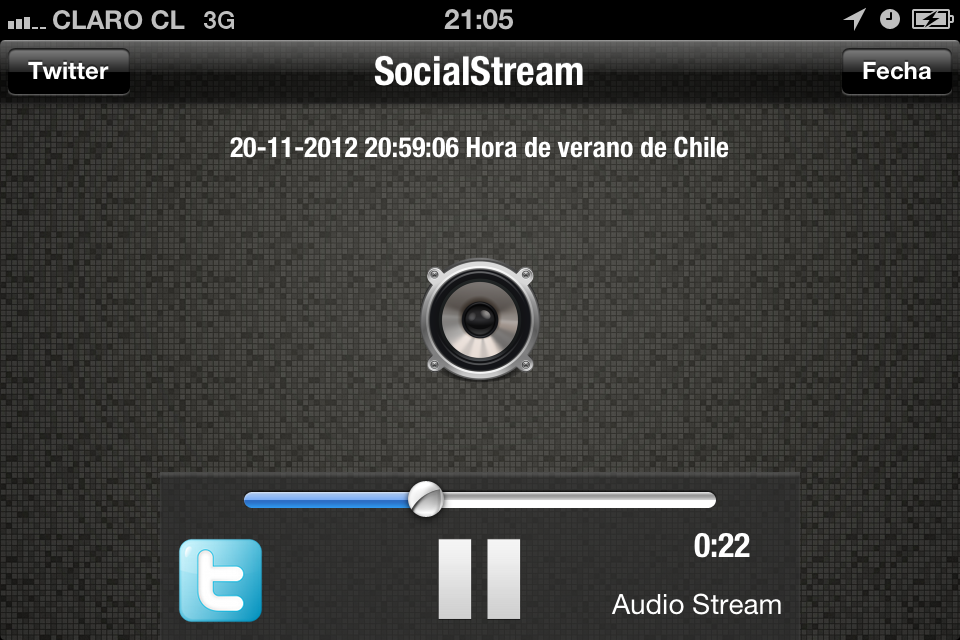
\includegraphics[scale=0.2]{imgs/cell-link-1.png} & 
	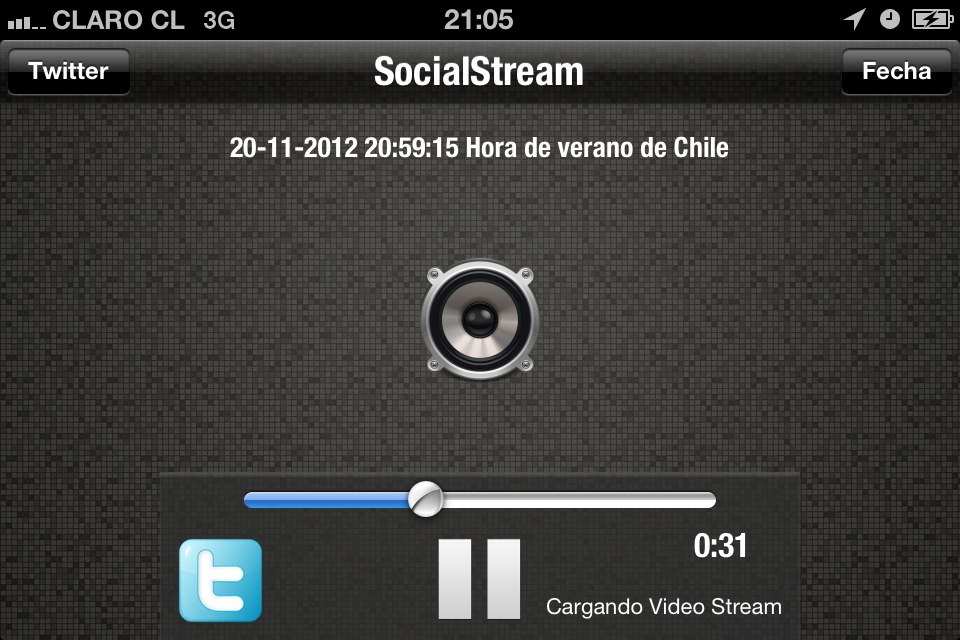
\includegraphics[scale=0.2]{imgs/cell-link-2.png} \\
	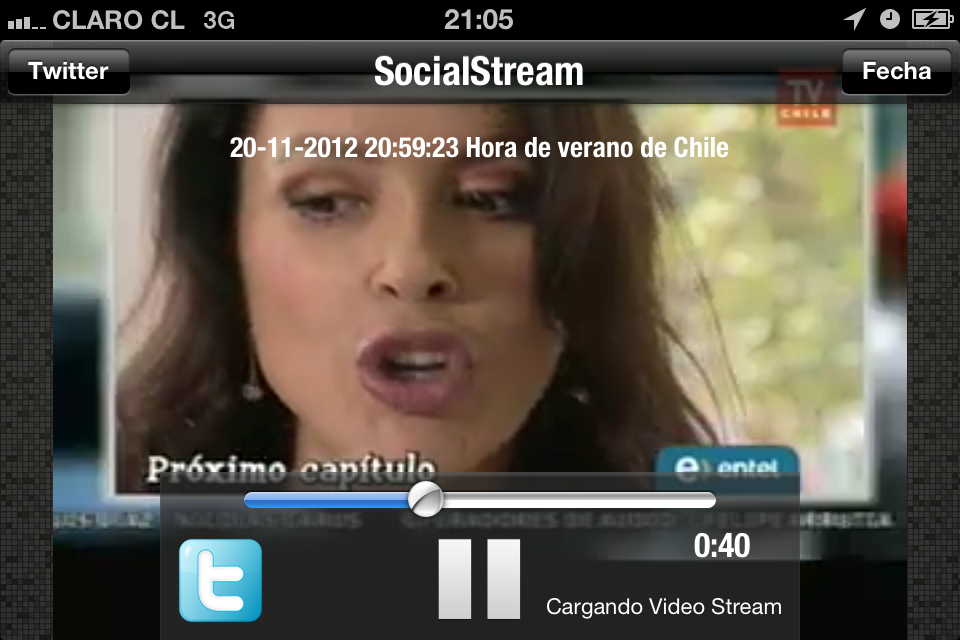
\includegraphics[scale=0.2]{imgs/cell-link-3.png} & 
	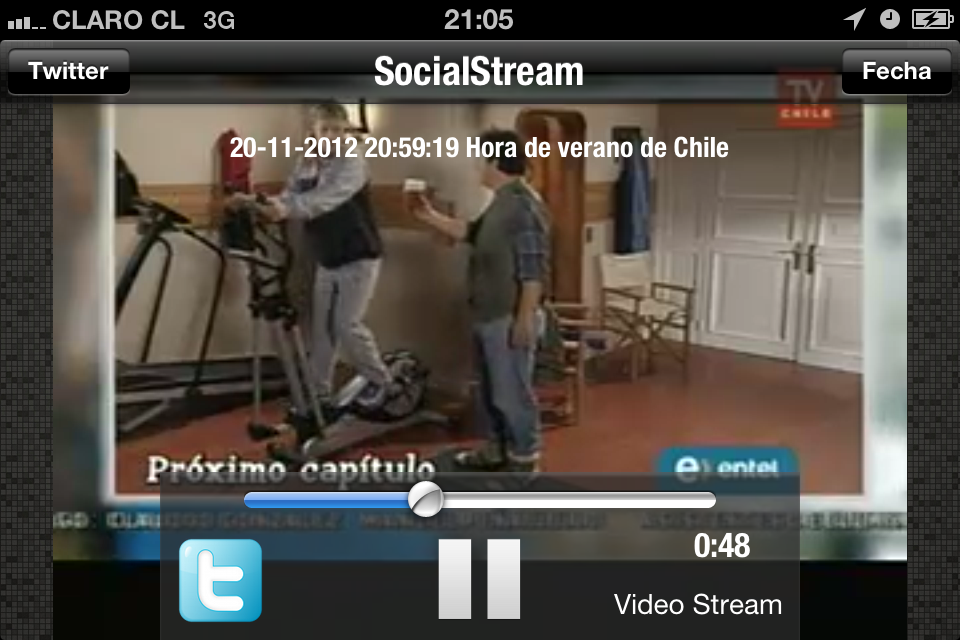
\includegraphics[scale=0.2]{imgs/cell-link-4.png} \\
	\end{tabular}
	\caption{iPhone reproduciendo stream de una fecha en particular a través de la red celular con enlace 3G.}
	\label{fig:cell-link}
\end{figure}

En la figura \ref{fig:cell-link} anterior se observa la secuencia de cambio de variante del stream. En la esquina inferior derecha del reproductor es posible observar el estado de las variantes, de izquierda a derecha pasa por los estados: Audio Stream, Cargando Video Stream, Video Stream. las imágenes 2 y 3 de la figura \ref{fig:cell-link} muestran el mismo estado a pesar que presentan distintas variantes, esto se debe a que para observar el estado de las variantes se  incorporó a la instancia de AVPlayer un observador del atributo \textit{tracks}, (página \pageref{item:kvo-tracks}, \textbf{Pistas de medios}) para comparar constantemente si alguna de las pistas son del tipo \textit{AVMediaTypeVideo}. 
En caso de observar cambios entre pistas que incluyen video a sólo pistas de audio y viceversa, se identifica el cambio de variante del stream.


\section{Cambio de transmisión mediante Twitter}
%- se revisa usando safari desktop con script que incluye player
%Gracias al modo desarrollador disponible en el navegador web para OS X Safari, es posible identificarse con el servidor utilizando un agente de usuario de Mobile Safari (iOS).

Para probar el cambio de stream a través de enlaces distribuidos por twitter se alojó el script \textbf{PHP} (\ref{subsec:php-redir}) en un servidor dispuesto por AltaVoz S.A. La ubicación de éste corresponde a \url{http://tsh.altavoz.net/twitter/index.php}.
El script utiliza los argumentos en la cadena de consulta \textbf{s} y \textbf{t} para generar un URL compatible si corresponde, o en caso contrario mostrar un mensaje de incompatibilidad.
  \subsection{Dentro de la aplicación}
  \label{subsec:ts-inside}
Se utiliza la llamada al método \textit{didSelectRowAtIndexPath:(NSIndexPath *)indexPath} gatillado al pulsar en un celda de la vista de tablas (fig. \ref{sshot-twitterclientvc}) utilizada para representar los Tweets asociados al \textit{hashtag} \textbf{\#SocialStream}. \\

\begin{figure}[H]
	\centering
	\begin{tabular}{cc}
	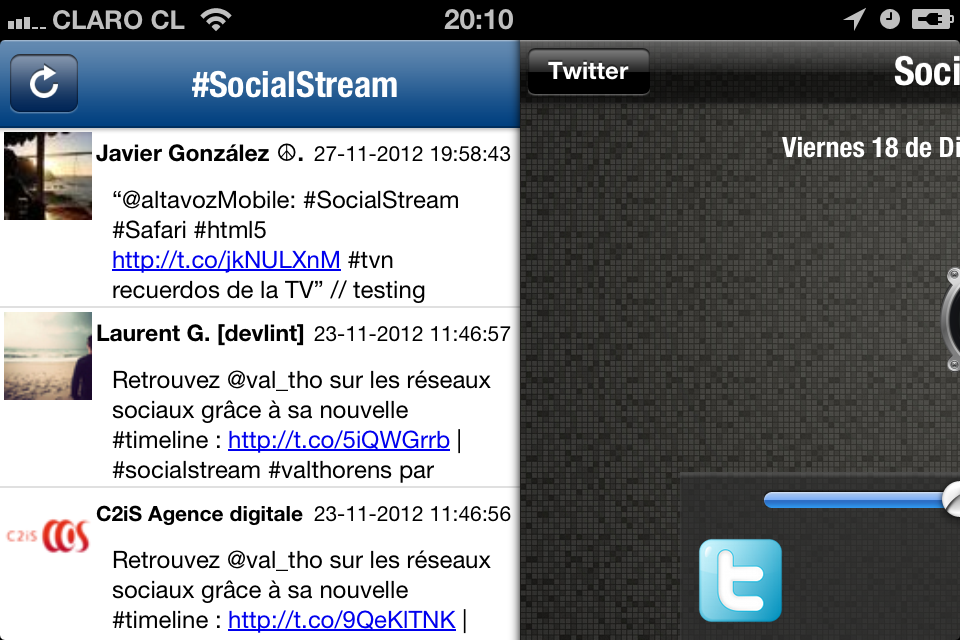
\includegraphics[scale=0.3]{imgs/twclient-list.png}
	\end{tabular}
	\caption{Vista de tabla con celdas compuestas de Tweets}
	\label{fig:twclient-list}
\end{figure}

El indice entregado al método se utiliza para identificar los datos del mensaje en el NSDictionary generado a partir del archivo JSON obtenido mediante Twitter Search API. De los datos contenidos en la instancia del diccionario \ref{tweet-json} se utiliza el valor de la clave \textbf{expanded\_url} para extraer la ruta del URL y generar un URL destinado al servicio \textbf{Bit.ly}.  \\

Del ejemplo en la figura \ref{fig:twclient-list} la primera celda presenta el dato \url{http://t.co/jkNULXnM}, el cual tiene como valor de \textbf{expanded\_url} asociado \url{http://bit.ly/Soxy8c}.

Esta ruta \textbf{Soxy8c}, que en realidad es el \textit{hash} bit.ly se utiliza para generar el URL:\\
\url{http://api.bit.ly/v3/expand?login=altavozchile&apikey=R_5947943f0ea1fe5b21df8269df2b4234&hash=Soxy8c}. \\

El resultado de esta llamada corresponde a un JSON que debe ser serializado a un NSDictionary y luego buscar en su clave \textbf{long\_url} los valores \textbf{s} y \textbf{t} de la cadena de consulta (fig. \ref{fig:twclient-debug}).\\

\begin{figure}[H]
	\centering
	\begin{tabular}{cc}
	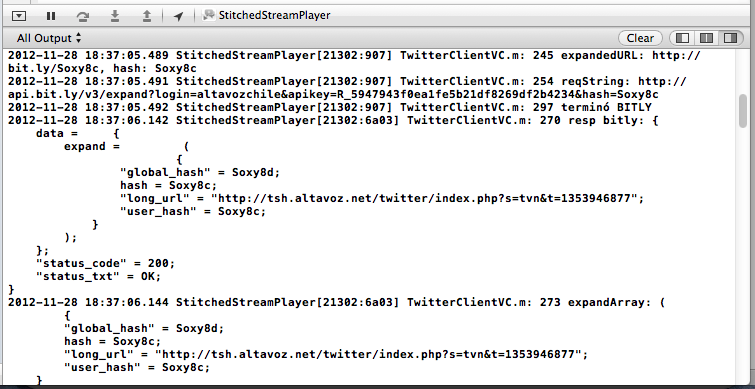
\includegraphics[scale=0.55]{imgs/twclient-debug.png}
	\end{tabular}
	\caption{Respuesta de bit.ly en la consola del depurador de Xcode.}
	\label{fig:twclient-debug}
\end{figure}


Si existen valores para \textbf{s} y \textbf{t} se procede a generar una notificación a la clase encargada de entregar el URL del stream a la instancia AVPlayer (fig. \ref{fig:twclient-results}, primera foto).

En caso contrario se presenta al usuario un aviso con la clase \textbf{UIAlertView} indicando que el URL contenido en ese mensaje no corresponde a un stream, dando la opción además de ser abierto en el navegador del sistema Mobile Safari mediante el método \textit{[[UIApplication sharedApplication] openURL:(NSURL*)url]}, logrando además que la aplicación se coloque en \textit{background} (fig. \ref{fig:twclient-results}, segunda foto).

\begin{figure}[H]
	\centering
	\begin{tabular}{cc}
	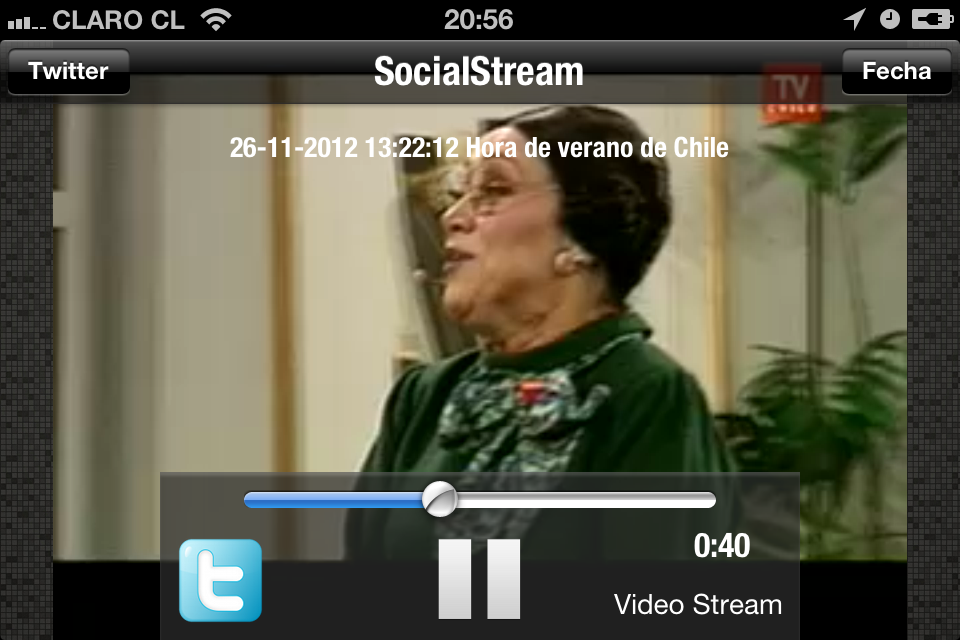
\includegraphics[scale=0.2]{imgs/twclient-stream.png} & 
	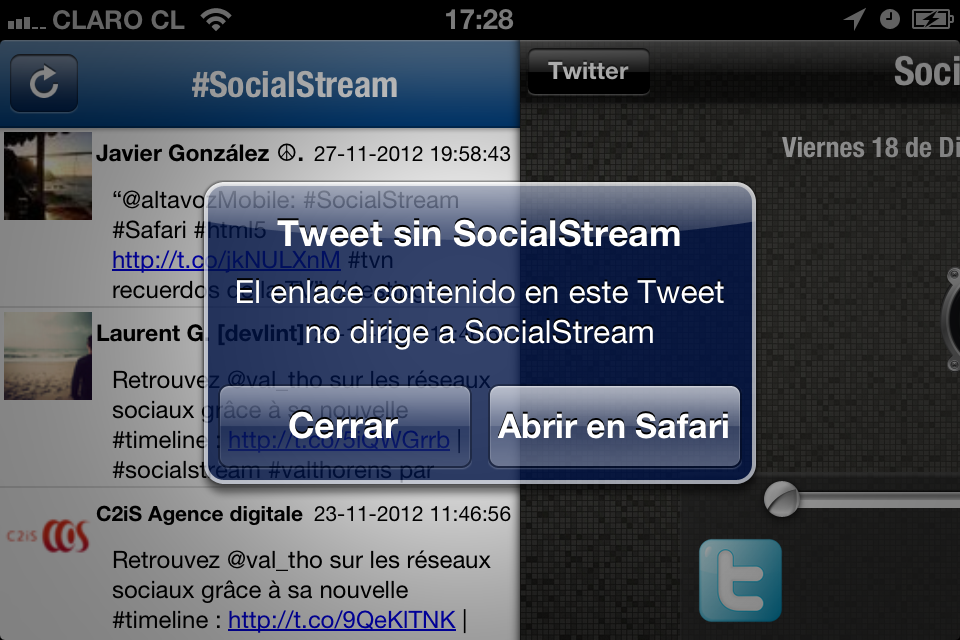
\includegraphics[scale=0.2]{imgs/twclient-nostream.png} \\
	\end{tabular}
	\caption{Distintos resultados de apertura de URLs contenidos en mensaje de Twitter}
	\label{fig:twclient-results}
\end{figure}


%	- debug viendo el cambio de tranmisión, URL generado y definiendo el mismo canal. manejo en caso de tweet sin enlace
%	se genera notificación interna con los componentes. ver que cambia el stream.

%{
%    "display_url" = "bit.ly/Soxy8c";
%    "expanded_url" = "http://bit.ly/Soxy8c";
%    indices =     (
%        46,
%        66
%    );
%    url = "http://t.co/jkNULXnM";
%}
%
%http://api.bit.ly/v3/expand?login=altavozchile&apikey=R_5947943f0ea1fe5b21df8269df2b4234&hash=Soxy8c
%
%    data =     {
%        expand =         (
%                        {
%                "global_hash" = Soxy8d;
%                hash = Soxy8c;
%                "long_url" = "http://tsh.altavoz.net/twitter/index.php?s=tvn&t=1353946877";
%                "user_hash" = Soxy8c;
%            }
%        );
%    };
%    "status_code" = 200;
%    "status_txt" = OK;
%}

  \subsection{Scheme registrado en iOS}
  
  Para revisar el comportamiento de la aplicación al ser lanzada por el sistema debido a la apertura de un URL que presenta el \textit{scheme} registrado, es necesario configurar el \textbf{Depurador} (\textit{debugger}) del entorno de desarrollo Xcode de forma que se encuentre a la espera de la apertura de la aplicación (fig. \ref{fig:xcode-waitforapp}), esto es diferente al comportamiento usual donde cada vez que se ejecuta en el compilador se lanza automáticamente en el dispositivo.\\
  
Este ajuste se logra editando el esquema (\textit{scheme}) de la compilación, no confundir con el esquema (\textit{scheme}) del URL. El entorno de desarrollo Xcode permite administrar distintos esquemas de compilación, siendo \textit{Build}, \textit{Run}, \textit{Analyze} y \textit{Archive} los más utilizados. Para mantener Xcode atento al lanzamiento de la compilación se debe editar el esquema \textbf{\textit{Run}} (ejecutar) como se muestra en la figura \ref{fig:xcode-debug-wait}.
  
%	- clientes de twitter en iPhone, twitter y Tweetbot, debug en el método e imprimir en consola la app que lo lanzó.  
%	- debug con app en background
%	- debug con app cerrada y a la espera que parta por otra aplicación
%	explicar que se detuvo la carga del stream cuando está cerrada y que se espera una notificacion de la carga de la UI antes de cargar el stream.

\begin{figure}[H]
	\centering
	\begin{tabular}{cc}
	
\includegraphics[scale=0.7]{imgs/xcode-waitforapp.png}
	\end{tabular}
	\caption{Entorno de desarrollo Xcode en modo de espera de apertura de la Aplicación.}
	\label{fig:xcode-waitforapp}
\end{figure}
    
\begin{figure}[H]
	\centering
	\begin{tabular}{cc}
	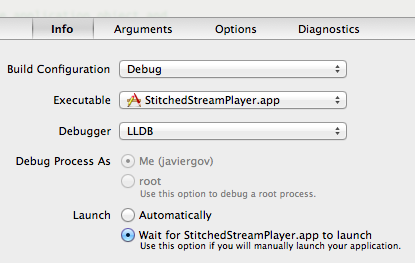
\includegraphics[scale=0.7]{imgs/xcode-debug-wait.png}
	\end{tabular}
	\caption{Configuración de Xcode para pruebas de lanzamiento de la aplicación por scheme.}
	\label{fig:xcode-debug-wait}
\end{figure}

Con esta configuración de depuración, ya es posible revisar el comportamiento con enlaces abiertos desde otra aplicación de iOS, como por ejemplo desde la aplicación de terceros Tweetbot. En la figura \ref{fig:tweetbot-sstream} al pulsar en el URL del tweet, el script desarrollado para la redirección (\ref{subsec:php-redir}) identifica el \textbf{Agente de Usuario} de la clase UIWebView presuntamente utilizada por Tweetbot para redirigir a un URL con el \textit{scheme} asociado por la aplicación cliente. El resultado se muestra en la segunda imagen donde el procedimiento consiste en generar una notificación a la clase que contiene la instancia de \textbf{AVPlayer} de forma que genere el URL necesario para reproducir el stream.\\

Al ser iniciada por esta vía, la aplicación gatilla el método de la clase delegada como instancia principal de la aplicación (\textit{AppDelegate}):\\

\textit{- (BOOL)application:(UIApplication*)application handleOpenURL:(NSURL*)url}\\

Dentro de esta llamada se generan las notificaciones encargadas de entregar un URL correspondiente al stream del instante compartido. Realizando pruebas se descubrió que la entrega de los datos a la aplicación no significaban el comportamiento esperado, es decir la visualización del stream en el preciso instante, esto debido a que el método encargado de manejar el URL se ejecutaba con anterioridad a los métodos de iniciación del reproductor, por lo tanto para asegurar la entrega de la información se programó un observador por notificación \cite{bib:ios-nsnotificationcenter} atento al aviso de carga del controlador de vistas que contiene la instancia del \textbf{AVPlayer} encargado de reproducir. \\

El aviso se realiza desde el método \textit{- (void)viewDidAppear:(BOOL)animated} del controlador de vistas, así es posible saber que las vistas, incluyendo la del reproductor, se han cargado en pantalla y proceder a entregar el URL del contenido.



\begin{figure}[H]
	\centering
	\begin{tabular}{cc}
	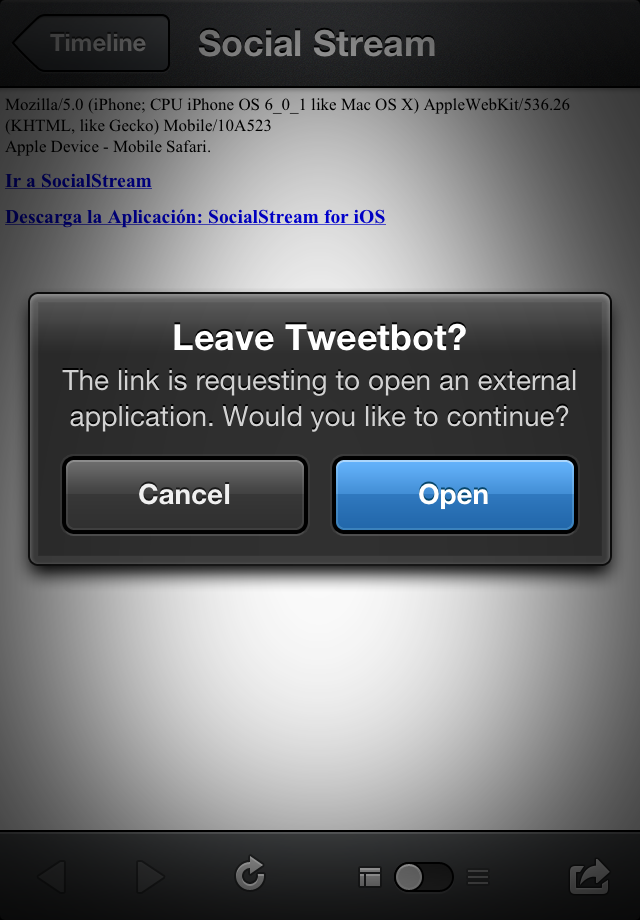
\includegraphics[scale=0.3]{imgs/tweetbot-sstream.png} &
	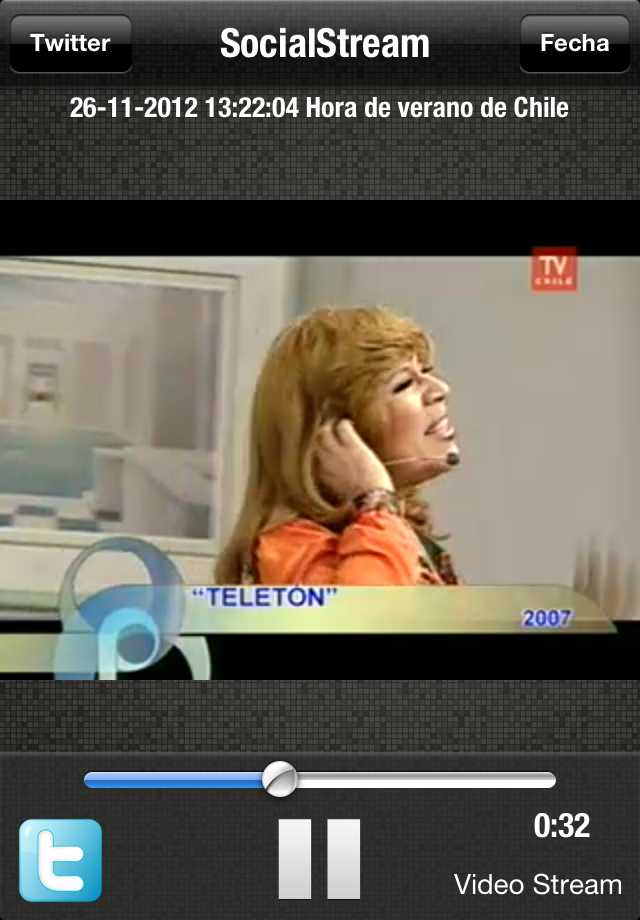
\includegraphics[scale=0.3]{imgs/tweetbot-appopened.png} \\
	\end{tabular}
	\caption{Solicitud de Tweetbot para abrir una aplicación externa y su posterior resultado.}
	\label{fig:tweetbot-sstream}
\end{figure}

\section{Enlaces Twitter en otros dispositivos}
A continuación se presentan los resultados de la apertura de URL compartidos a través de la aplicación cliente a través de distintas plataformas.
%	pantallazos de páginas de error, el por qué y cómo se entregan según el script, no se revisa internet explorer porque se utilizaron navegadores compatibles con OS X.
	
  \subsection{PC Escritorio}
  Se presentan capturas de pantalla de la reacción del script desarrollado con distintos navegadores web compatibles con Mac OS X. Ese es el motivo por cual Internet Explorer no aparece en estos resultados, ya que desde su versión 5.2.3 lanzada el 16 de junio de 2003 \cite{bib:mac-iexplorer} no existe soporte para sistema operativo nombrado.

    \subsubsection{Safari}
El navegador web Safari al ser producto de las tecnologías desarrolladas por Apple es compatible para la reproducción de streams HLS. Para mostrar el contenido se utilizó la marca de HTML5  \textless VIDEO\textgreater \ con la lista de reproducción generada por el script php como fuente de video. El resultado es el reproductor visto en la figura \ref{fig:uagent-safari}.\\

Además también en pruebas se utilizó el widget dispuesto por Twitter \cite{bib:twitter-widget} para embeber tweets relacionados a cierto hashtag, en este caso: \#SocialStream. El uso de este widget solo fue por motivos de experimentación.
%      safari muestra un player html5
%    foto del player

  \begin{figure}[H]
	\centering
	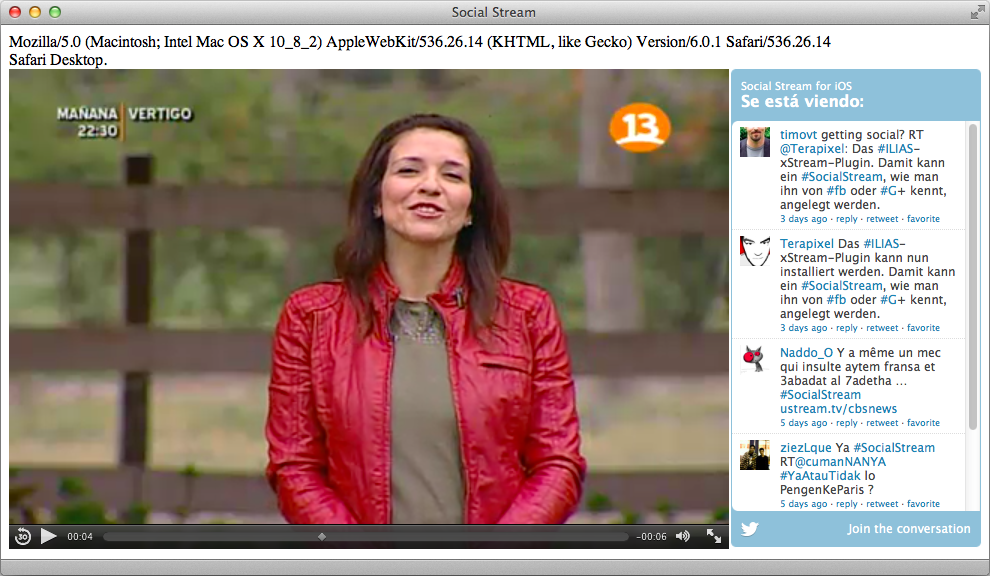
\includegraphics[scale=0.4]{imgs/uagent-safari.png} 
	\caption{Apertura de enlace compartido desde la aplicación cliente en Safari.}
	\label{fig:uagent-safari}
\end{figure}  
    
    \subsubsection{Chrome}
  \begin{figure}[H]
	\centering
	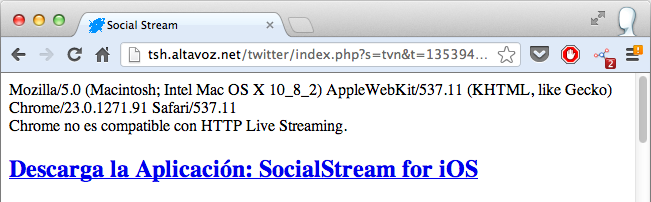
\includegraphics[scale=0.6]{imgs/uagent-chrome.png} 
	\caption{Apertura de enlace compartido desde la aplicación cliente en Google Chrome.}
	\label{fig:uagent-chrome}
\end{figure}  
    \subsubsection{Firefox}
  \begin{figure}[H]
	\centering
	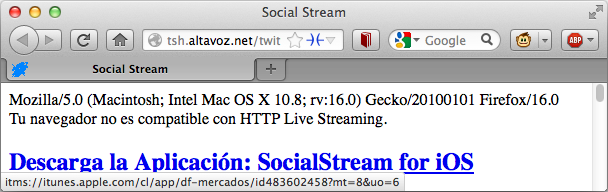
\includegraphics[scale=0.6]{imgs/uagent-firefox.png} 
	\caption{Apertura de enlace compartido desde la aplicación cliente en Mozilla Firefox.}
	\label{fig:uagent-firefox}
\end{figure}  
    \subsubsection{Opera}
  \begin{figure}[H]
	\centering
	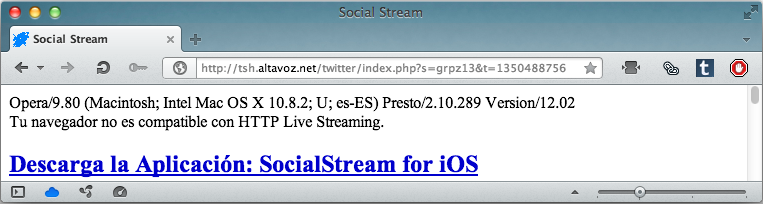
\includegraphics[scale=0.55]{imgs/uagent-opera.png} 
	\caption{Apertura de enlace compartido desde la aplicación cliente en Opera.}
	\label{fig:uagent-opera}
\end{figure}  
  \subsection{Android y otros móviles incompatibles}
  En el caso del celulares con el sistema operativo Android se presenta el mensaje de la figura \ref{fig:uagent-android}. Si bien desde la versión 4.0, Android OS es compatible con HTTP Live Streaming, es necesario desarrollar una aplicación similar a la hecha para iOS.
 \begin{figure}[H]
	\centering
	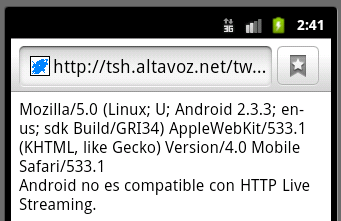
\includegraphics[scale=0.7]{imgs/uagent-android.png} 
	\caption{Apertura de enlace compartido desde la aplicación cliente en Safari.}
	\label{fig:uagent-android}
 \end{figure}  

%  pantallazo del cell de la esperanza
%  explicar que tampoco es compatible con HLS, por lo menos 2.3, 4.0 ICS en adelante es compatible, pero para reproducir el stream se debe desarrollar una aplicación cliente similar a la hecha en iOS

\section{Comparación con SocialStream Flash}

En las figuras \ref{sshot_iOS_sstream} y \ref{fig:eag-player} se puede observar el reproductor del stream de video distribuido a través del protocolo RTMP. El reproductor fue desarrollado por un alumno de la Universidad Técnica Federico Santa María para demostrar la capacidad de cambiar el tiempo del contenido en un reproductor de video desarrollado con las tecnologías de Adobe Flash.

\begin{figure}[H]
	\centering
	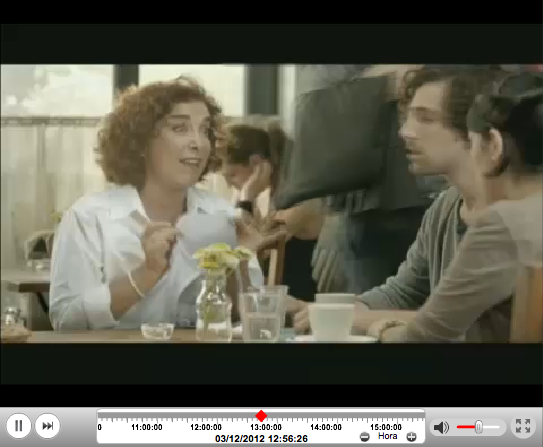
\includegraphics[scale=0.6]{imgs/eag-player.png} 
	\caption{Reproductor Flash para Timeshift en Navegador web Safari.}
	\label{fig:eag-player}
\end{figure}  

En las figuras \ref{fig:twclient-results} y \ref{fig:cell-link} se presenta el reproductor desarrollado por el autor de este documento como resultado del proyecto del tema de memoria.\\

En esta sección se destacan las diferencias de usabilidad de los reproductores para el usuario final, más allá de la gran diferencia que el reproductor de la figura \ref{fig:eag-player} y el desarrollado en iOS se utilizan en plataformas distintas. 

\begin{itemize}
\item \textbf{Protocolo:} El reproductor Flash utiliza protocolo RTMP mientras que el reproductor para iOS recibe el contenido a través de HTTP Live Streaming.
\item \textbf{Salto de Tiempo:} la forma de saltar en el tiempo en el reproductor flash precisa de clicks con mouse, ya sea para cambiar la escala de su linea de tiempo como para moverse el punto central de reproducción, lo cual dificulta en gran medida el consumo del contenido mientras se busca otro instante.\\

En el caso del reproductor iOS se utiliza el control explicado en la sección \ref{subsec:datepicker}, que permite elegir un tiempo en especifico pulsando el botón \textbf{Cargar} o cancelar la selección de fecha pulsando fuera del área del selector sin intervenir el contenido en reproducción.

\item \textbf{Entrega de contenido:} El contenido en el reproductor Flash presenta una mayor exactitud al elegir un tiempo en especifico, esto debido a que la segmentación del video es cada 5 segundos. En el caso de HTTP Live Streaming es recomendado por los ingenieros de Apple que desarrollaron el protocolo, utilizar 10 segundos como mínimo para cada segmento de video o audio. El motivo de esta recomendación es evitar paralizaciones (\textit{stalls}) en la transmisión a través de redes celulares \cite{bib:tensec-targetduration}.\\

\item \textbf{Redes Sociales:} Esta fue una característica adicional a la solución de permitir transmisión con saltos en el tiempo en iOS. Durante el desarrollo de la aplicación cliente se descubrió el potencial de realizar cambios de lista de reproducción del protocolo HTTP Live Streaming a través de cadenas de consulta de los URLs y compartir el contenido a través de redes. En el caso del reproductor Flash el cambio temporal se realiza a través de la comunicación bidireccional del protocolo RTMP mediante la función \textit{seek} enviada desde el cliente (especificación RTMP \cite{bib:rtmp-specs} sección 4.2.7 - \textit{seek}).
\end{itemize}
%mostrar player original de eduardo, la diferencia de la linea de tiempo, el salto de tiempo, la exactitud y que no es tan exacto porque los segmentos son de 10 segundos

%la linea de tiempo difiere con una representación gráfica, se utilizó el control de fecha para simplificar el punto a elegir, además la linea de tiempo precisa de mouse over para mostrar datos y en el caso táctil difiere mucho.


